\documentclass[12pt]{article} 
\usepackage[margin=1in]{geometry}
\usepackage{enumitem} %% for custom list
\usepackage{graphicx} %% for images
\usepackage{multirow} %% for tables
\usepackage{bytefield} %% for drawing packet structure
\usepackage{color} %% for color when drawing packet structure
%\usepackage{wrapfig} %% used to wrap img around text: https://goo.gl/SrlHQI

\usepackage{graphicx} %% used to split page in two columns
\usepackage{multicol}

\usepackage[dvipsnames]{xcolor} %% to use with VerbatimInput to import stuff from text file
\usepackage{fancyvrb}

%\usepackage{bigints}  %% for integrals

% used for tabbed spacing
%\newcommand{\itab}[1]{\hspace{0em}\rlap{#1}}
%\newcommand{\tab}[1]{\hspace{.4\textwidth}\rlap{#1}}

% using \code{come code monospaced}
\def\code#1{\texttt{#1}}

% redefine \VerbatimInput
\RecustomVerbatimCommand{\VerbatimInput}{VerbatimInput}%
{fontsize=\footnotesize,
 %
 frame=lines,  % top and bottom rule only
 framesep=2em, % separation between frame and text
 rulecolor=\color{Gray},
 %
 %label=\fbox{\color{Black}data.txt},
 %labelposition=topline,
 %
 commandchars=\|\(\), % escape character and argument delimiters for commands within the verbatim
 commentchar=*        % comment character
}

\begin{document}
\date{}
%\author{Andrea Ghizzoni \\
%some other info}
\title{\vspace{-11ex}} %% used for no title
 
\maketitle

\section{Livello di Rete}\label{livello-di-rete}
Nel modello TCP/IP, il livello di rete viene detto \textbf{livello internet} oppure \textit{livello di internetworking} 
e si occupa della consegna \textit{point-to-point} delle informazioni; in altre parole permette la trasmissione dei dati 
attraverso reti anche di diversa natura. A questo livello \'e necessario conoscere solamente l'indirizzo 
sorgente e destinazione degli host, in quanto tutta la semantica della comunicazione tra processi remoti ed eventuale 
controllo di flusso viene gestita dal livello superiore.

Sono necessari quindi dei meccanismi che permettano al livello di rete di scoprire la quali host sono connessi al 
proprio tratto di rete, in modo da sapere il percorso \textit{"migliore"} per il \textbf{Routing} 
\textit{(Instradamento)} dei dati, e un modo univoco di identificare tutte le interfacce di rete sulla stessa, per 
essere in grado di eseguire il \textbf{Forwarding} \textit{(Inoltro)} correttamente alla destinazione.

Il protocollo utilizzato nella IPS che implementa tutte le funzionalit\'a appena descritte \'e chiamato \textbf{IP} 
\textit{(Internet Protocol)}. Inoltre definisce lo standard per gli apparati di rete che hanno lo specifico compito di 
connettere le reti tra loro e di inoltrare il traffico in modo ottimale a seconda della destinazione del pacchetto, 
questi \textit{relay system} vengono chiamati \textbf{Router} \textit{(Commutatori)}.

Pi\'u precisamente la PDU del livello di rete viene chiamata \textbf{Datagram} \textit{(datagramma)}.
\begin{center}
	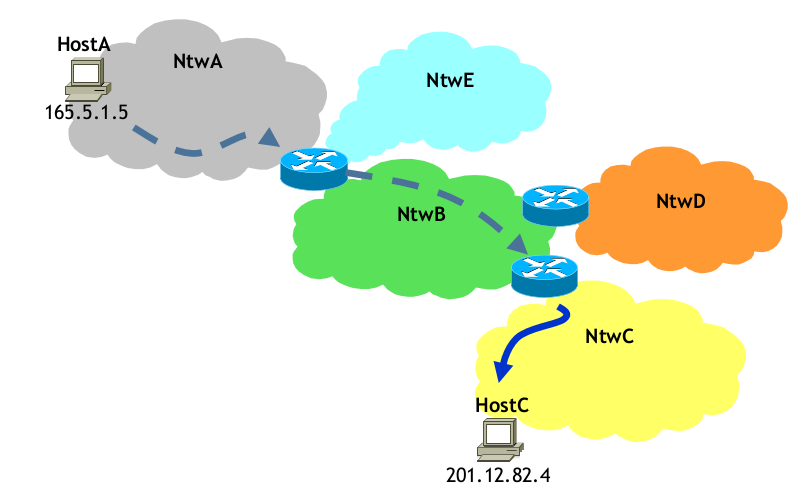
\includegraphics[scale=0.35]{livello_di_rete-img1.png}
\end{center}
Come si vede dall'immagine soprastante, \code{HostA} vuole comunicare con \code{HostC} ma appartengono a reti diverse. 
In questo caso il livello di rete di \code{HostA} sa che tutti i dati con una destinazione diversa da \code{NtwA}, 
dovranno essere consegnati al router pi\'u vicino, in modo che ci penser\'a lui ad inoltrarlo correttamente a 
\code{NtwC} (consegna \textit{indiretta}). Ora il router decider\'a quale percorso utilizzare per inoltrare 
correttamente il datagramma, utilizzando le tabelle di routing precedentemente calcolate, fino a raggiungere il router 
che \textit{"conosce"} la rete del destinatario originale della comunicazione, \code{HostC}. L'ultimo passo \'e di 
consegnare direttamente i datagrammi a \code{HostC} (consegna \textit{diretta}).

\clearpage
\subsection{Riassumendo}\label{livello-di-rete-riassumendo}
Riassumendo, le funzioni fondamentali del livello di rete:
\begin{itemize}
	\item \textbf{Routing:} calcolare il percorso \textit{"migliore"} dalla sorgente alla destinazione utilizzando degli 
	       appositi algoritmi di Routing
	\item \textbf{Forwarding:} lo spostamento dei datagrammi da una linea in ingresso linea d'uscita
	\item \textbf{Indirizzamento:} l'identificazione in modo univoco di ogni host sullo stesso tratto di rete
	\item \textbf{Tunnelling:} incapsulamento ulteriore dei datagrammi per permettere il loro transito su determinati 
	      tipi di rete.
\end{itemize}

\subsection{Internetworking}\label{livello-di-rete-internetworking}
Di seguito verranno analizzati i problemi che sorgono quando si collegano tra loro due o pi\'u reti che supportano 
protocolli e/o richiedono caratteristiche differenti.

Per connettere reti diverse le possibilit\'a sono due: si possono costruire sistemi che traducano i datagrammi per un 
dato tipo di rete oppure aggiungere un livello comune a tutte. La seconda soluzione \'e quella adottata nella IPS  con 
il protocollo IP.

\subsubsection{Tunneling}\label{livello-di-rete-internetworking-tunnelling}
Nel caso in cui due host vogliano comunicare tra di loro, ma sono separati da un tratto di rete che non supporta gli 
stessi protocolli della rete del sorgente e della destinazione, il \textbf{Tunneling} \textit{(fare da tunnel)}
riesce ad incapsulare tutti i datagrammi della sorgente nel payload dei datagrammi che possono transitare su quel tratto 
di rete, quindi estrarli e ricomporli una volta arrivati dall'altro cado della rete.

L'esempio seguente si riferisce al tunneling dei datagrammi IPv6 attraverso una rete che supporta solo IPv4.
\begin{center}
	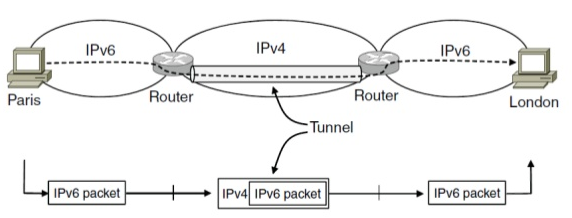
\includegraphics[scale=0.65]{livello_di_rete-img3.png}
\end{center}

\subsubsection{Frammentazione dei datagrammi}\label{livello-di-rete-internetworking-frammentazione}
Ogni rete impone una dimensione massima ai datagrammi che possono circolare al suo interno. Questo pu\'o dipendere da 
vari fattori come: hardware degli apparati di rete, sistemi operativi, standard internazionali ecc\dots

La tendenza \'e di trasmettere datagrammi di grandi dimensioni per ridurre l'overhead, ma \'e possibile che debbano
transitare attraverso una rete che non li supporta, ovvero che la rete consente una \textbf{MTU} \textit{(Maximum 
Transfer Unit)} minore della precedente. In questo caso il datagramma deve essere suddiviso in frammenti, inviati
poi come un nuovi datagrammi a livello di rete.

Il problema principale nell'utilizzo di questo approccio \'e proprio corretta gestione dei frammenti da parte del 
router, quindi si possono attuale le seguenti scelte:
\begin{itemize}[noitemsep]
    \item frammentare del datagramma all'inizio della rete con MTU pi\'u piccola e ricostruzione all'uscita: questo 
          comporta un peggioramento delle prestazioni perch\'e \'e possibile che si creino coni di bottiglia
    \item non ricomporre il datagramme e continuare a trasmettere i frammenti lungo il tratto di rete rimasto: in questo 
          modo non vengono sprecate risorse per la ricomposizione ma, necessita che il protocollo in uso preveda la 
          frammentazione tramite opportuni campi nell'header.    
\end{itemize}
Per risolvere definitivamente il problema \'e necessario non frammentare i datagrammi alla sorgente, infatti IP prevede 
il protocollo \textbf{MTU Path Discovery} per scoprire la dimensione minima della MTU lungo il tratto di rete tra 
sorgente e destinazione. Il suo funzionamento \'e molto semplice: un host invia un datagramma impostato come non 
frammentabile alla destinazione, se un tratto di rete intermedio non supporta quella dimensione risponder\'a con
un datagramma di errore contenente la sua massima MTU supportata.

Fermo restando che il percorso preso dai datagrammi non \'e necessariamente detto che rimanga tale per tutta 
la durata della trasmissione.



\clearpage
\section{Router}
I router, o \textit{commutatori}, sono dei relay system che lavorano esclusivamente a livello di rete, non hanno bisogno 
dei livelli soprastanti che gestiscano connessioni e perdita di pacchetti, in quanto il loro compito \'e di permettere 
l'inoltro dei datagrammi attraverso sottoreti diverse. Per riuscire in questo \'e necessario che il router abbia:
\begin{itemize}[noitemsep]
	\item una interfaccia di rete per ogni sottorete a cui \'e collegato\footnote{oppure una sola interfaccia divisa 
	      logicamente a livello software}
	\item la conoscenza dei suoi router \textit{"vicini"}
	\item un algoritmo decisionale per l'inoltro dei datagrammi attraverso il percorso \textit{"migliore"}
\end{itemize}

\subsection{Commutazione di Pacchetto - Store and Forward}\label{router-commutazione-di-pacchetto}
Tutti i router implementano la tecnica chiamata \textbf{Store and Forward} \textit{(Salva e Inoltra)} che permette di 
salvare temporaneamente il pacchetto in memoria per controllare il checksum e l'indirizzo di destinazione, e 
successivamente decidere qual'\'e il prossimo \textbf{Hop} \textit{(Salto)}, ovvero quale router, inoltrarlo.

\begin{center}
	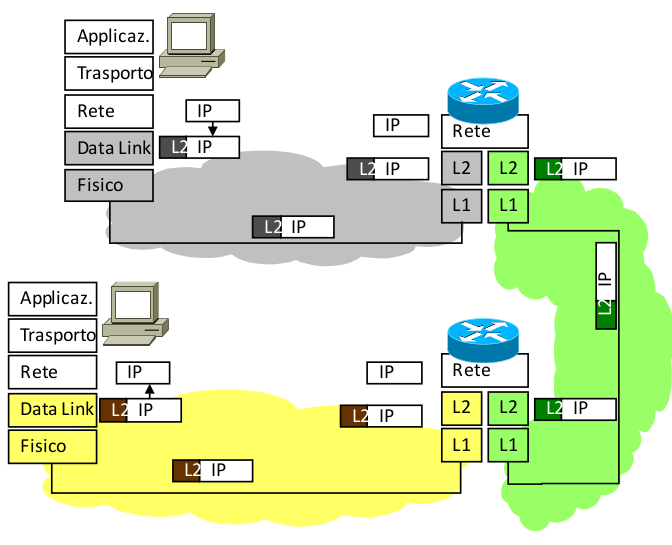
\includegraphics[scale=0.4]{livello_di_rete-img2.png}
\end{center}
In figura si nota come i router conoscano a quali sottoreti sono collegati e, in base all'indirizzo di rete associato 
all'indirizzo IP di destinazione e la maschera di sottorete, riescano a capire a quale router inoltrare il datagramma. Il 
router in alto conosce che per tutti i datagrammi in entrata dalla sottorete \textit{grigia} verso la sottorete 
\textit{gialla}, dovr\'a inoltrarli al router sulla sottorete \textit{verde}, in quanto lui non ha conoscenza di come 
raggiungere direttamente la sottorete \textit{gialla}.

\clearpage
\subsection{Instradamento - Routing}\label{router-instradamento}
Il meccanismo di \textbf{routing} \textit{(instradamento)} dei pacchetti, \'e necessario per non creare una connessione
fisica tra sorgente e destinatario per ogni coppia di host in internet, in quanto permette al commutatore di decidere 
quale percorso \'e pi\'u \textit{"conveniente"} far percorrere ad un dato datagramma. A tale scopo si rende necessario
la realizzazione di software adatto a scegliere il miglior percorso, o la migliore direzione, per minimizzare la
latenza ed impedire la congestione degli apparati di rete.

Un \textbf{Algoritmo di Routing} \'e, quindi, quella parte del software di rete che si occupa capire a quali sottoreti \'e 
collegato il commutatore per poi prendere decisioni sull'inoltro dei datagrammi ingresso.

La parte cruciale del software \'e la capacit\'a di adattarsi ai cambiamenti della rete: congestione, perdita di un 
collegamento fisico oppure aggiunta di un nuovo commutatore. A fronte dei cambiamenti, ogni router deve mantenere 
aggiornato una tabella di "costi" per ogni sottorete a cui \'e collegato, dove per "costi" si intende una unit\'a di 
misura in base alla quale pu\'o prendere una decisione sull'inoltro dei datagrammi. Questa tabella viene chiamata 
\textbf{Routing Table} \textit{(Tabella di Inoltro)}.

\'E facile immaginare che non \'e pensabile impostare una tabella di routing statica, per ogni commutatore in internet, in 
quanto, per stessa definizione di internet, \'e una rete estremamente dinamica, con collegamenti che si aggiungono e si 
tolgono continuamente. Quindi i router devono adattarsi a questa caratteristica intrinseca della rete.
\begin{center}
	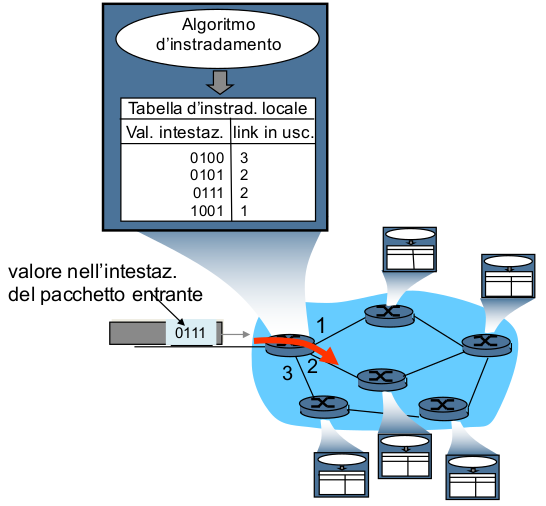
\includegraphics[scale=0.5]{livello_di_rete-img7.png}
\end{center}
Come si vede dall'immagine ogni router ha calcolato la propria tabella di instradamento in funzione delle sottoreti a lui 
collegate. Nel momento in cui riceve un datagramma in ingresso, viene interrogata per sapere in quale link in uscita 
inoltrarlo.

\clearpage
\subsection{Distribuzione delle Tabelle di Routing}\label{router-distribuzione-tabelle-routing}
Il problema dell'instradamento dei pacchetti si riduce essenzialmente a come diffondere le informazioni dei link locali dei 
router a tutti gli altri, in modo tale che ogni commutatore conosca ogni possibile destinazione. Queste problematiche 
vengono affrontate in vario modo dai protocolli e dagli algoritmi seguenti.

\subsubsection{Distance Vector Routing}\label{router-distribuzione-tabelle-routing-distance-vector}
Il primo algoritmo \'e basato sul \textit{Vettore delle Distanze} dove ogni router misura, il \textit{"costo"} dei 
collegamenti tra lui e tutti i suoi vicini tramite il numero di \textbf{hop} \textit{(salti)}, producendo cos\'i il vettore 
delle distanze. Ovviamente verr\'a mantenuta l'associazione \code{vicino-costo}. Per mettere a conoscenza gli altri router 
che attraverso di lui si possono raggiungere alcune destinazioni ad un certo costo, invia a tutti i suoi vicini il suo 
vettore delle distanze.

A questo punto, il procedimento avviene contemporaneamente per tutti i router collegati, quindi \'e necessario decidere 
come aggiornare il proprio vettore delle distanze in funzione di quello ricevuto. Quindi Possono accadere i seguenti casi:
\begin{itemize}[noitemsep]
	\item una destinazione \code{X} che prima era irraggiungibile (costo infinito) ora \'e raggiungibile tramite un vicino 
	      \code{Y} a costo \code{k}, quindi aggiorno il mio vettore nella posizione della destinazione \code{X} scrivendo 
	      \code{{Y},{k+n}}, dove \code{n} \'e il costo per andare da \code{X} a \code{Y}
	\item una destinazione \code{X} \'e raggiungibile attraverso il vicino \code{Y} con un costo \code{k} inferiore a 
	      quello che ho attualmente, quindi aggiorno il mio vettore alla posizione della destinazione \code{X} scrivendo 
	      \code{{Y},{k+n}}, dove \code{n} \'e il costo per andare da \code{X} a \code{Y}
	\item una destinazione \code{X} non \'e raggiungibile, oppure ha un costo superiore al mio attraverso il vicino 
	      \code{Y}, quindi mantengo la mia distanza
\end{itemize}
Ogni aggiornamento del vettore delle distanza locale al router provoca la sua trasmissione a tutti i vicini.

\'E ragionevole pensare che questo tipo di algoritmo non termini mai, ovvero aggiornamenti provocano ritrasmissioni, che 
provocano aggiornamenti ecc\dots Questo tipo di problema prende il nome di \textit{count to infinity} ma fortunatamente 
accade solo in determinate circostanze e normalmente \textit{converge} ad una situazione stabile anche se lentamente.

Ci\'o nonostante \'e stato previsto che i pacchetti di aggiornamento vengano inviati con il campo \code{TTL} pari a 15, 
limitando il diametro massimo della rete.

Un'implementazione dell'algoritmo basato sul vettore delle distanze \'e \textbf{RIP} \textit{(Routing Information 
Protocol)}.

\paragraph{Riassumendo}\label{router-distribuzione-tabelle-routing-distance-vector-riassumendo}
\begin{itemize}[noitemsep]
	\item ogni router ha una visione ristretta della topologia della rete
	\item non necessita di una nozione condivisa di distanza
	\item costruzione del percorso minimo partendo dalla destinazione e andando verso le sorgenti in modo additivo.
\end{itemize}

\clearpage
\paragraph{Esempio}\label{router-distribuzione-tabelle-routing-distance-vector-esempio}
Di seguito viene mostrato un grafo i quali nodi sono i router e gli archi sono i collegamenti tra essi. La tabella accanto ai 
nodi raffigura la routing table ad ogni iterazione del protocollo ed \'e cos\'i composta: \code{X} \'e la colonna 
destinazione dove \code{X} \'e il nome del nodo, \code{dist} \'e la distanza, \code{NH} \'e il next hop.

\begin{multicols}{2}[\columnsep4em] 	
	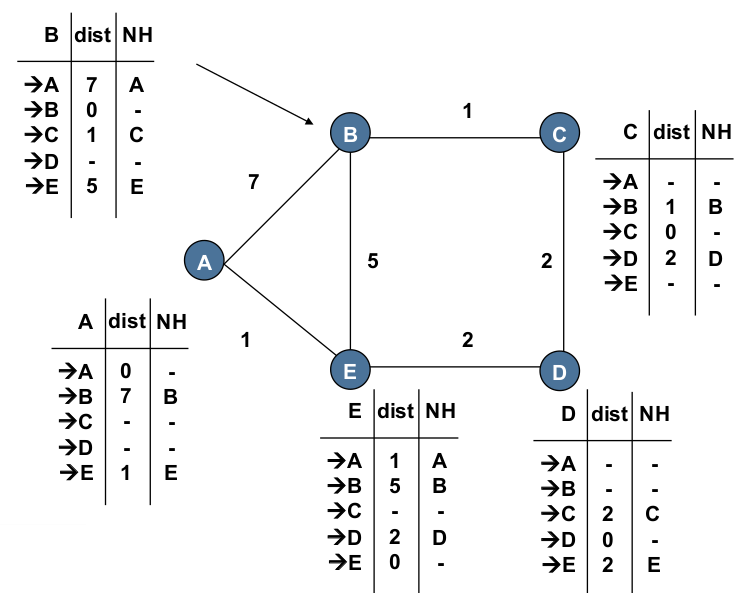
\includegraphics[scale=0.3]{livello_di_rete-img8.png}
	\columnbreak
	
	I protocolli di tipo distance vector partono dalla seguente situazione: ogni router \'e a conoscenza solo dei propri 
	vicini e della loro distanza.
	
	Ovviamente verr\'a descritto il funzionamento per il nodo \code{D}, ma contemporaneamente avviene in tutti i nodi.
\end{multicols}
\begin{multicols}{2}[\columnsep4em] 	
	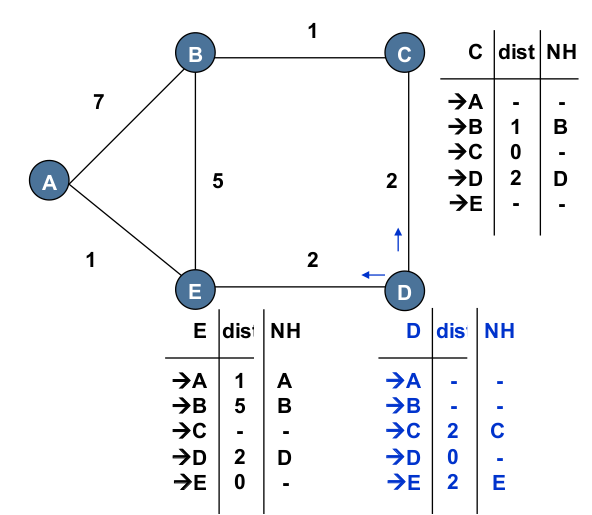
\includegraphics[scale=0.3]{livello_di_rete-img9.png}
	\columnbreak
	
	Il router \code{D} una volta costruito il suo vettore delle distanze lo distribuisce ai suoi vicini \code{C} e \code{E}
\end{multicols}
\begin{multicols}{2}[\columnsep4em] 	
	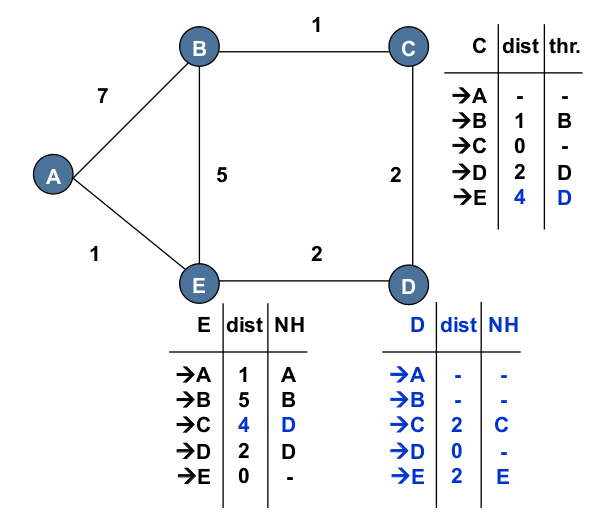
\includegraphics[scale=0.3]{livello_di_rete-img10.png}
	\columnbreak
	
	Il router \code{C} riceve il vettore e nota che prima non riusciva a raggiungere \code{E} ma, tramite \code{D} ora riesce 
	a raggiungerlo a costo 
	\begin{center}
		2 (\code{C-D}) + 2 (\code{D-E}) = 4
	\end{center}
	
	Al router \code{E} accade lo stesso evento del router \code{C}: riceve il vettore delle distanze da \code{D} e nota che 
	ora riesce a raggiungere \code{C} tramite \code{D} a costo 
	\begin{center}
		2 (\code{E-D}) + 2 (\code{D-C}) = 4
	\end{center}
\end{multicols}
\clearpage
\begin{multicols}{2}[\columnsep4em] 	
	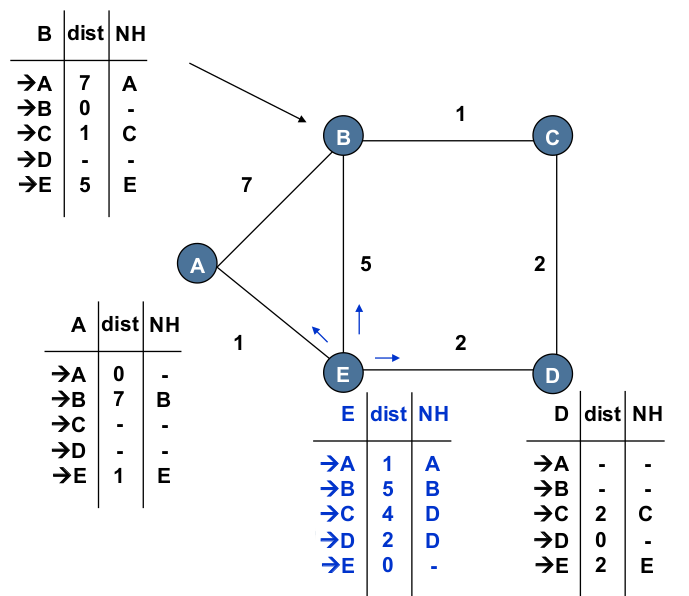
\includegraphics[scale=0.3]{livello_di_rete-img11.png}
	\columnbreak
	
	Ora concentriamo l'attenzione sul nodo \code{E}. Dopo aver ricevuto i vettore delle distanze ed aggiornato il suo lo 
	invia ai suoi vicini \code{B}, \code{A} e \code{D}. 
\end{multicols}
\begin{multicols}{2}[\columnsep4em] 	
	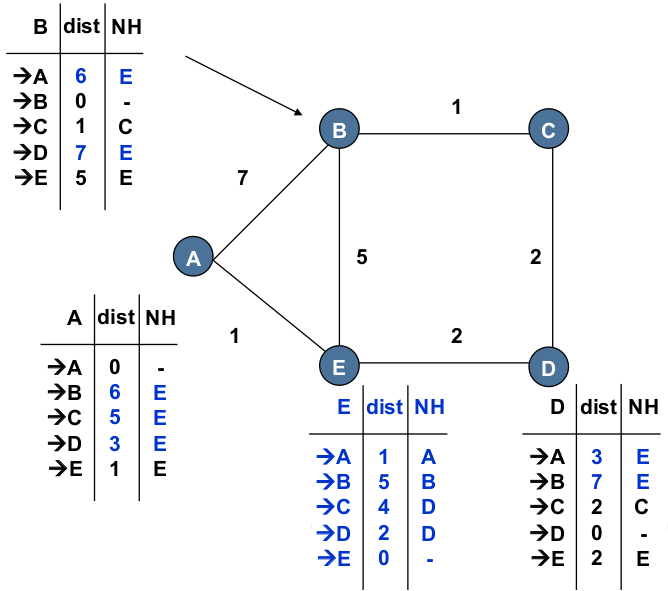
\includegraphics[scale=0.3]{livello_di_rete-img12.png}
	\columnbreak
	
	I router \code{B}, \code{A} e \code{D} ricevono il nuovo vettore delle distanze di \code{E} ed aggiornano le voci con 
	solo i valori che portano ad un costo minore tramite il router \code{E}: il router \code{B} aggiorna \code{A} e \code{D} 
	rispettivamente con
	\begin{center}
		5 (\code{B-E}) + 1 (\code{E-A}) = 6\\
		5 (\code{B-E}) + 2 (\code{E-D}) = 7		
	\end{center}
	
	Il router \code{A} aggiorna \code{B}, \code{C} e \code{D} rispettivamente con
	\begin{center}
		1 (\code{A-E}) + 5 (\code{E-B}) = 6\\
		1 (\code{A-E}) + 4 (\code{E-C}) = 5\\
		1 (\code{A-E}) + 2 (\code{E-D}) = 3		
	\end{center}
	
	Ed infine il router \code{D} aggiorna \code{A} e \code{B} rispettivamente con
	\begin{center}
		2 (\code{D-E}) + 1 (\code{E-A}) = 3\\
		2 (\code{D-E}) + 5 (\code{E-B}) = 7		
	\end{center}
\end{multicols}
Ovviamente il processo continuerebbe fino alla convergenza del sistema ma si nota chiaramente che ci sono molti scambi di 
vettori che potrebbero essere evitati.


\clearpage
\subsubsection{Link State Routing}\label{router-distribuzione-tabelle-routing-link-state-routing}
Il secondo algoritmo usato per la distribuzione e la creazione delle tabelle di routing prende il nome di \textbf{Link Stat 
Routing} \textit{(Instradamento sullo stato dei collegamenti)}. Viene comunemente pi\'u utilizzato di Distance Vector 
perch\'e permette un tempo di convergenza minore e permette al router di avere una visione globale della topologia della 
rete.

I passi dell'algoritmo quindi sono (per ogni router):
\begin{itemize}[noitemsep]
	\item \textbf{scoprire l'indirizzo di rete dei propri vicini}: ogni router invia in broadcast un datagramma 
	      \code{ICMP Hello} e memorizzer\'a tutti gli indirizzi di rete delle risposte
	\item \textbf{misurazione del costo dei collegamenti}: sfruttando il punto precedente e attraverso una speciale 	
	      funzione riesce a ricavare un costo per il collegamento verso ogni destinazione
	\item \textbf{costruzione dei pacchetti che contengono lo stato di collegamento}: dopo aver risposto ai datagrammi 	
	      degli altri router vicini, crea un datagramma contenente il suo stato dei collegamenti
	\item \textbf{distribuzione lo stato dei collegamenti}: utilizzando il flooding distribuisce lo stato dei collegamenti 
          \footnote{per evitare la distribuzione infinita si utilizza un campo che viene usato come numero di sequenza; 
          ogni router tiene traccia della coppia \code{sorgente-sequenza}, cos\'i se riceve un pacchetto con numero di 
          sequenza inferiore lo scarta, altrimenti lo propaga flooding}
	\item \textbf{calcolo dei percorsi}: una volta ricevute le informazioni sullo stato del collegamento dagli altri
		  router, \'e possibile costruire un grafo della rete
\end{itemize}
Una volta terminato l'algoritmo, il router avr\'a creato un grafo che gli dar\'a la visione globale della topologia della 
rete, quindi non pi\'u limitata alla conoscenza del prossimo router per minimizzare il numero di salti per arrivare alla 
destinazione. 

Per la creazione della vera tabella di routing viene quindi eseguito l'algoritmo di Dijkstra per la ricerca dei cammini 
minimi sul grafo della rete per ogni possibile destinazione.

L'implementazione usata in Internet che utilizza il protocollo di tipo link state \'e \textbf{OSPF} \textit{(Open Shortest 
Path First)}.

\paragraph{Riassumendo}\label{router-distribuzione-tabelle-routing-link-state-routing-riassumendo}
\begin{itemize}[noitemsep]
	\item ogni router ha la visione globale della topologia della rete
	\item necessita di una nozione condivisa di misurazione della distanza
	\item costruzione del percorso minimo attraverso delle informazioni locali
\end{itemize}

\clearpage
\paragraph{Esempio}\label{router-distribuzione-tabelle-routing-dijkstra-esempio}
Di seguito viene riporta la topologia di una rete di router con i relativi costi dei collegamenti. Questo grafo si pu\'o 
supporre che sia memorizzato nel nodo \code{A} e di eseguire l'algoritmo di Dijkstra per il calcolo dei cammini minimi.
\begin{center}
	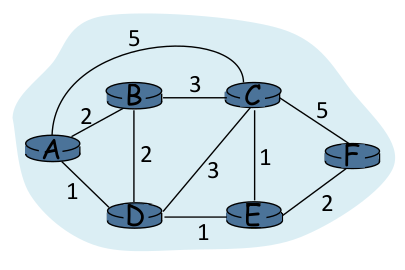
\includegraphics[scale=0.6]{livello_di_rete-img14.png} % 0.6 for impagination
\end{center}
Nella tabella sottostante vengono proposti tutte le iterazioni dell'algoritmo. Sulla colonna \code{set(N)} vengono inseriti i 
nodi scelti a costo minimo per ogni iterazione, invece le restanti rappresentano ogni router nel grafo, senza la sorgente 
\code{A}, nella forma "\code{D(X),p(X)}" che significa \textit{distanza da} \code{X} \textit{attraverso il predecessore} 
\code{X}.

Allo Step 0 la tabella risulta popolata solo con i dati dei vicini del router \code{A}
\begin{center}
\renewcommand{\arraystretch}{1.2}% spacing between rows
\begin{tabular}{ c r r r r r r }
	\code{Step} & \code{set(N)} & \code{D(B),p(B)} & \code{D(C),p(C)} & \code{D(D),p(D)} & \code{D(E),p(E)} & 
	\code{D(F),p(F)}\\ \hline
	0 &      A & 2,A              & 5,A              & {\color{red}1,A} & $\infty$         & $\infty$         \\ \hline
\end{tabular}
\end{center}
Ad ogni iterazione si considera la colonna con il costo minimo\footnote{\label{note1}in caso di parit\'a scelgo quella che mi aggrada di pi\'u}, in questo caso il nodo \code{D} che ha costo \code{1}. Quindi 
si crea una nuova riga dove si aggiunge al \code{set(N)} il nodo \code{D}.

\begin{center}
\renewcommand{\arraystretch}{1.2}% spacing between rows
\begin{tabular}{ c r r r r r r }
	\code{Step} & \code{set(N)} & \code{D(B),p(B)} & \code{D(C),p(C)} & \code{D(D),p(D)} & \code{D(E),p(E)} & 
	\code{D(F),p(F)}\\ \hline
	0 &      A & 2,A              & 5,A              & {\color{red}1,A} & $\infty$         & $\infty$         \\ \hline
	1 &     AD & X                & Y                & Z                & W                & H                \\ \hline
\end{tabular}
\end{center}
Ora, ogni volta che si aggiunge nuovo router al \code{set(N)} si devono calcolare le nuove distanze minime che sono 
raggiungibili dai router attualmente presenti nel \code{set(N)}: in questo caso al posto di \code{X, Y, Z, W} e \code{H} 
andranno calcolati:

\begin{itemize}[noitemsep]
	\item \code{X}: per arrivare a \code{B} posso scegliere:
	\begin{itemize}[noitemsep]
		\item \code{(A-B)} a costo \code{2} passando da \code{A}, quindi \code{2,A} (costo della riga sopra)
		\item \code{(A-D-B)} a costo \code{1+2=3} passando da \code{D}, quindi \code{3,D}	
	\end{itemize}
	\item \code{Y}: per arrivare a \code{C} posso scegliere:
	\begin{itemize}[noitemsep]
		\item \code{(A-C)} a costo \code{5} passando da \code{A}, quindi \code{5,A} (costo della riga sopra)
		\item \code{(A-D-C)} a costo \code{1+3=4} passando da \code{D}, quindi \code{4,D}	
	\end{itemize}
	\item \code{Z}: questo elemento rappresenta la colonna del router \code{D}, che ho gi\'a nel \code{set(N)}, quindi non 
	      faccio niente
	\item \code{W}: per arrivare a \code{E} posso scegliere:
	\begin{itemize}[noitemsep]
		\item attraverso \code{A} non riesco ad arrivare ad \code{E}, quindi $\infty$
		\item \code{(A-D-E)} a costo \code{1+1=2} passando da \code{D}, quindi \code{2,D}	
	\end{itemize}
	\item \code{H}: per arrivare a \code{F} non ho nessuna scelta, ne attraverso \code{A} ne \code{D}, quindi $\infty$
\end{itemize}
Per ogni possibile scelta elencata sopra scelgo quella con costo minimo\footnotemark[\ref{note1}], quindi la riga dello Step 
1 risulter\'a

\begin{center}
\renewcommand{\arraystretch}{1.2}% spacing between rows
\begin{tabular}{ c r r r r r r }
	\code{Step} & \code{set(N)} & \code{D(B),p(B)} & \code{D(C),p(C)} & \code{D(D),p(D)} & \code{D(E),p(E)} & 
	\code{D(F),p(F)}\\ \hline
	0 &      A & 2,A              & 5,A              & {\color{red}1,A} & $\infty$         & $\infty$         \\ \hline
	1 &     AD & 2,A              & 4,D              & ==               & {\color{red}2,D} & $\infty$         \\ \hline
\end{tabular}
\end{center}
A questo punto si ricomincia tutto il procedimento appena illustrato con il router con costo minimo preso dalla riga appena 
creata, ovvero \code{E}. 

Una volta raggiunti tutti i nodi la tabella risulter\'a
\begin{center}
\renewcommand{\arraystretch}{1.2}% spacing between rows
\begin{tabular}{ c r r r r r r }
	\code{Step} & \code{set(N)} & \code{D(B),p(B)} & \code{D(C),p(C)} & \code{D(D),p(D)} & \code{D(E),p(E)} & 
	\code{D(F),p(F)}\\ \hline

	0 &      A & 2,A              & 5,A              & {\color{red}1,A} & $\infty$         & $\infty$         \\ \hline
	1 &     AD & 2,A              & 4,D              & ==               & {\color{red}2,D} & $\infty$         \\ \hline
	2 &    ADE & {\color{red}2,A} & 3,E              & ==               & ==               & 4,E              \\ \hline
	3 &   ADEB & ==               & {\color{red}3,E} & ==               & ==               & 4,E              \\ \hline
	4 &  ADEBC & ==               & ==               & ==               & ==               & {\color{red}4,E} \\ \hline
	5 & ADEBEF & ==               & ==               & ==               & ==               & ==               \\ \hline
\end{tabular}
\end{center}
A questo punto quello che si \'e ottenuto \'e il \textit{minimum spanning tree} del grafo di partenza, ovvero l'albero di 
copertura minimo, che poi verr\'a utilizzato per la creazione della tabella di routing del nodo \code{A}.

\begin{center}
	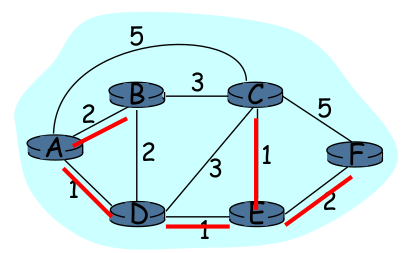
\includegraphics[scale=0.5]{livello_di_rete-img15.png}
\end{center}

\clearpage
\subsubsection{Flooding}\label{router-distribuzione-tabelle-routing-flooding}
Il \textbf{Flooding} \textit{(Inondazione)} non rientra nelle categorie di algoritmi atti alla creazione o alla 
distribuzione delle tabelle di routing, ma \'e semplicemente una tecnica che distribuzione delle informazioni.

Un router che distribuisce delle informazioni in flooding non deve fare altro che riceverle da un'interfaccia di rete e 
replicarla su tutte le altre interfacce. Il nome deriva proprio da questa caratteristica. 

Ovviamente si generano molti informazioni duplicate, che vengono gestiti tramite il campo \code{TTL} di IP oppure tramite 
numeri di sequenza opportunamente impostati.

Il vantaggio nell'utilizzo del flooding \'e la sua intrinseca semplicit\'a di implementazione e robustezza, sceglie sempre 
il percorso pi\'u breve perch\'e prova ogni possibile percorso in parallelo.

\subsection{Instradamento Globale}\label{router-instradamento-tra-as}
Gli algoritmi di instradamento presentati finora avevano la caratteristica di memorizzare uno \textit{"stato"} della rete, 
ovvero i collegamenti o l'intera topologia. In realt\'a non \'e mai possibile che i router odierni memorizzino milioni e 
milioni di informazioni relative a tutte le possibili sottoreti esistenti, oltretutto il traffico generato dalle 
informazioni di aggiornamento non lascerebbero capacit\'a di elaborazione del router per i dati utente.

Per questi motivi viene adottata una sistema di instradamento \textbf{gerarchico}, ovvero vengono raggruppati i router, 
tipicamente presenti su ogni territorio nazionale e gestiti da un ente governativo, per formare un \textbf{Autonomous 
System o AS} \textit{(Sistema Autonomo)}, dove viene applicato OSPF come algoritmo di instradamento.

Questa organizzazione porta il vantaggio immediato che tutti i router all'interno dell'AS avranno delle tabelle 
di instradamento relativamente piccole, dovute al numero di sottoreti presenti, ma nasce il problema di come collegare vari 
AS tra di loro. Ogni sistema autonomo mette a disposizione dei router particolari, identificati come \textbf{Border Router} 
\textit{(Commutatori di Confine)}, che hanno il compito specifico di instradare tutti il traffico in entrata e in uscita 
tra gli AS. Il collegamento tra border router viene chiamato \textbf{Backbone Area} \textit{(Area di Dorsale)}.

Ovviamente non ha senso che nelle tabelle di instradamento dei border router compaiano tutte le possibili sottoreti 
presenti negli altri AS, sarebbe una contraddizione. In questo caso \'e necessario che i border router effettuino un 
instradamento di livello \textit{"superiore"}, ovvero che non si basino pi\'u sul numero di sottoreti da attraversare per 
raggiungere la destinazione, ma sul percorso tra AS. 

Purtroppo le tabelle di instradamento che definiscono questo percorso non sono il risultato di un algoritmo per la ricerca 
del cammino minimo tra quest'ultimi, ma frutto di accordi economico-commerciali tra gli enti dei vari paesi che le 
gestiscono. In questo mondo pu\'o succedere che datagrammi provenienti da AS \textit{"amici"} prendano un percorso 
preferenziale rispetto a datagrammi di AS \textit{"non-amici"}.

L'implementazione del protocollo usato dai border router \'e chiamato \textbf{BGP} \textit{(Border Gateway Protocol)}.



\clearpage
\section{Spazio di indirizzamento in IP}\label{spazio-indirizzamento-in-ip}
La parte riguardante lo spazio di indirizzamento, \'e la parte cruciale di tutto il sistema di Internet. Tutti gli host 
e i router devono usare uno schema di indirizzamento unico e uniforme.

Attualmente esiste lo standard \textbf{IP} con due versioni: \textbf{IPv4} e \textbf{IPv6}; entrambi completamente 
supportati in Internet ma il secondo \'e stato creato per rimpiazzare il primo in quanto fornisce opzioni pi\'u avanzate 
e uno spazio di indirizzi maggiore.

\subsection{Indirizzi IPv4}\label{pazio-indirizzamento-in-ip-indirizzi-ipv4}
Gli indirizzi IPv4, o pi\'u semplicemente IP, sono numeri a 32 bit assegnate ad ogni interfaccia di rete. Per una 
migliorane la comprensione e la gestione viene usata la notazione \textbf{Dotted Decimal}, ovvero l'indirizzo viene 
suddivisa in 4 gruppi da 8 bit ciascuno, ed espressi in forma decimale. Nella tabella seguente sono riportati degli 
esempi:
\begin{center}
	\begin{tabular}{ |c|c| }
		\hline
		\textbf{Numero binario a 32bit} & \textbf{Notazione Dotted Dicimal} \\
 		\hline
 		\code{10000001 00110100 00000110 00000000}  & \code{129.52.6.0}  \\ 
 		\code{11000000 00000101 00110000 00000011}  & \code{192.5.48.3}  \\ 
 		\code{00001010 00000010 00000000 00100101}  & \code{10.2.0.37}  \\  
 		\hline
	\end{tabular}
\end{center}
Ma gli indirizzi IP non sono sufficienti per identificare univocamente un'interfaccia di rete. Si prenda in 
considerazione il seguente esempio: un azienda ha bisogno di connettere alla rete un gruppo di computer, per gli 
standard di internet \'e necessario che abbiamo tutti un indirizzo univoco, quindi sar\'a necessario acquistare 
dall'ICANN un numero congruo di indirizzi. Questo esempio mette in luce che assegnare un indirizzo unico a livello 
mondiale ad un comune terminale aziendale \'e un problema sia per chi vuole creare la sua rete privata sia per il numero 
esiguo di indirizzi pubblici.

Per risolvere questo genere di problematiche si \'e deciso di utilizzare un nuovo numero a 32 bit chiamato 
\textbf{Sub-Net Mask} \textit{(Maschera di Sottorete)} che, invece di identificare un host, identifica un intera rete, 
in modo da capire se un dato indirizzo IP appartiene o meno a quella sottorete.

In altre parole agisce come un \textit{"raggruppatore"} di indirizzi, in modo da suddividere un solo IP pubblico in 
tante sottoreti diverse; questo porta il vantaggio che lo stesso indirizzo pu\'o essere utilizzato in sottoreti 
differenti.

La suddivisione avviene tramite \textbf{AND logico bit-a-bit} tra un indirizzo IP e la sua maschera di sottorete.
\paragraph{Esempio:} L'indirizzo \code{128.208.1.14} con la maschera di sottorete \code{255.255.255.0} indica:
\begin{center}
	\begin{tabular}{l|l}
		\code{128.208.1.14}                  & indirizzo IP \\
		\code{255.255.255.0}                 & maschera di sottorete \\
		\code{\underline{128.208.1}.0}       & risultato dell'AND bit-a-bit tra indirizzo e maschera\\
		\code{\underline{128.208.1}.0 - \underline{128.208.1}.255}   & possibili indirizzi utilizzabili dagli host \\
	\end{tabular}
\end{center}

\paragraph{Esempio:} L'indirizzo \code{128.208.1.14} con la maschera di sottorete \code{255.255.254.0} indica:
\begin{center}
	\begin{tabular}{l|l}
		\code{128.208.1.14}                  & indirizzo IP \\
		\code{255.255.254.0}                 & maschera di sottorete \\
		\code{\underline{128.208.0}.0}       & risultato dell'AND bit-a-bit tra indirizzo e maschera\\
		\code{\underline{128.208.0}.0 - \underline{128.208.1}.255}   & possibili indirizzi utilizzabili dagli host \\
	\end{tabular}
\end{center}

Come si nota dagli esempi precedenti l'indirizzo \code{128.208.1.14} identifica due interfacce di rete diverse, il che 
va contro il concetto stesso di unicit\'a degli indirizzi. Ma grazie alle sottoreti \'e possibile riutilizzarlo, 
risparmiando una quantiat\'a considerevole di indirizzi pubblici.

La maschera di sottorete, quindi, divide la parte di indirizzo IP che identifica univocamente la rete, chiamato 
\textbf{NetID} \textit{(Prefisso)}, dalla parte riservata agli host, chiamata \textbf{HostID} \textit{(Suffisso)}. La 
NetID rimane uguale per tutti gli host di una data rete, per definizione; a livello globale invece, deve essere 
assegnata da un'autorit\'a in modo tale da non creare conflitti in fase di routing. Mentre per l'assegnamento degli 
HostID \'e lasciato ai progettisti della rete stessa.

\'E possibile scrivere la maschera di sottorete in dotted decimal, ma la notazione pi\'u compatta e comoda risulta la 
\textbf{Slash Notation}, ovvero riportare quanti bit sono impostati a \code{1} dopo il carattere \code{"/"}. Alcuni 
esempi:
\begin{center}
	\begin{tabular}{ |c|c| }
		\hline
		\textbf{Notazione Dotted Dicimal} & \textbf{Slash Notation}\\
 		\hline
 		\code{255.255.255.0} & \code{/24} \\ 
 		\code{255.255.254.0} & \code{/23} \\ 
 		\code{255.255.240.0} & \code{/20} \\  
 		\hline
	\end{tabular}
\end{center}
Esistono tuttavia degli indirizzi \textit{"speciali"} che ogni sottorete possiede e non \'e possibile assegnarli agli 
host in quanto identificano:
\begin{itemize}[noitemsep]
	\item \textbf{Indirizzo di Rete:} ottenuto con l'AND logico bit-a-bit tra l'indirizzo IP e la maschera di sottorete
	\item \textbf{Indirizzo di Broadcast:} ultimo indirizzo ottenibile nella sottorete, usato per la trasmissione dei 
	      datagrammi a tutti gli host
	\item \textbf{Indirizzo di Loop-Back:} generalmente \'e \code{127.0.0.1}
\end{itemize}

\paragraph{Esempio:} La scrittura \code{128.208.0.14/24} indica:\\
\begin{center}
	\begin{tabular}{l|l}
		\code{128.208.0.14}    & indirizzo dell'host    \\
		\code{255.255.255.0}   & maschera di sottorete  \\
		\code{128.208.0.0}     & indirizzo di rete      \\
		\code{128.208.0.255}   & indirizzo di broadcast \\
		\code{128.208.0.1 - 128.208.0.254} & spazio di indirizzamento per gli host \\ 
	\end{tabular}
\end{center}

\clearpage
\subsection{Indirizzi Pubblici e Privati}\label{pazio-indirizzamento-in-ip-indirizzi-pubblici-privati}
L'utilizzo della maschera di sottorete ha portato alla luce la distinzione tra un indirizzo pubblico, assegnato 
dall'autorit\'a competente, e indirizzo privato, ottenuto dalla suddivisione della rete in tante sottoreti.

Sono stati definiti anche degli standard sulla forma che dovrebbe assumere un indirizzo privato:
\begin{center}
	\begin{tabular}{l}
		\code{10.0.0.0  - 10.255.255.255}   \\
		\code{172.16.0.0 - 172.16.255.255}  \\
		\code{192.168.0.0 - 192.168.255.255}\\
	\end{tabular}
\end{center}

Quello che accade oggigiorno \'e che la scarsit\'a di indirizzi pubblici ha portato a suddividere le reti sempre pi\'u 
gerarchicamente. In questo modo un ISP pu\'o acquistare un limitato numero di indirizzi e suddividerlo tra i suoi router 
dei abbonati. Infatti ogni abbonato possiede una piccola rete interna privata con un solo indirizzo pubblico assegnato 
al suo router.

Con questo tipo di rete si crea il problema di far comunicare due host in sottoreti diverse con potenzialmente lo stesso 
indirizzo IP. Esistono due soluzioni al problema: il \textbf{NAT} \textit{(Network Address Translation)} o il 
\textbf{Proxy}.

\subsubsection{NAT}\label{pazio-indirizzamento-in-ip-indirizzi-pubblici-privati-nat}
Il sistema NAT permette di sostituire a tutti i datagrammi del livello rete l'indirizzo privato della sottorete interna 
con l'indirizzo pubblico del router usato per la connessione ad Internet. In altre parole agisce da 
\textit{"traduttore"} degli indirizzi privati in indirizzi pubblici e viceversa. 

In questo modo tutte i datagrammi in uscita verso Internet avranno come sorgente l'indirizzo del router, mascherando 
l'indirizzamento interno della rete privata.

Per via che questo meccanismo funzioni il router ha bisogno di mantenere una tabella, chiamata \textbf{Natting Table} 
\textit{(Tabella di NAT)}, per salvare tutte le informazioni necessarie alla traduzione degli indirizzi. Solitamente 
ogni elemento della tabella \'e cosi composto:
\begin{center}
	\code{SRC IP - DST IP - SRC PORT - DST PORT - PROTOCOL}
\end{center}

\clearpage
\paragraph{Esempio}
\begin{center}
	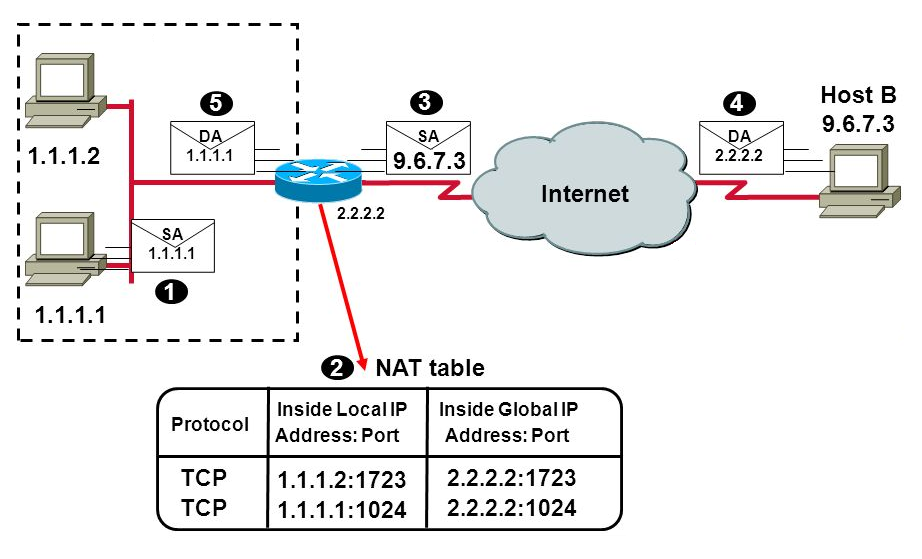
\includegraphics[scale=0.5]{livello_di_rete-img6.png}
\end{center}
Come si vede dall'immagine precedente, l'host nella rete privata con indirizzo \code{1.1.1.1} cerca di comunicare con 
l'host con l'indirizzo \code{9.6.7.3}. Come prima cosa controlla se l'indirizzo di destinazione appartiene alla sua 
sottorete eseguendo l'AND bit-a-bit con l'indirizzo di destinazione e la sua maschera di sottorete. Verificato che il 
risultato non \'e uguale al suo indirizzo di rete, invia i datagrammi al router NAT. 

A questo punto viene aggiunto una riga nella tabella di NAT con le informazioni del flussi di datagrammi in uscita, 
viene costruito un nuovo datagramma cambiando l'indirizzo sorgente in quello del router \code{2.2.2.2} ed infine viene 
inviato in Internet.

Come si vede dall'immagine l'Host B non risponde con l'indirizzo di destinazione della rete interna private 
\code{1.1.1.1} ma con quello del router \code{2.2.2.2}. A questo punto eseguir\'a una traduzione inversa, sempre grazie 
alla tabella di NAT e inoltrer\'a il datagramma alla destinazione interna.

\subsubsection{Proxy}\label{pazio-indirizzamento-in-ip-indirizzi-pubblici-privati-proxy}
Un altro modo per permettere ad host con indirizzi privati di comunicare con Internet \'e quello di utilizzare un Proxy.
Un proxy \'e un software installato su un host server ad indirizzo pubblico che rimane in ascolto delle richieste di 
livello applicativo da parte di un host interno alla sottorete, quindi esegue una richiesta identica verso Internet con 
il proprio indirizzo sorgente.

Alla ricezione della risposta, il proxy la invier\'a all'applicazione originaria sull'host interno della sottorete 
cambiando l'indirizzo sorgente con il proprio. In questo modo l'host non avr\'a alcun modo di sapere quale host remoto 
ha risposto alla sua richiesta, ma sapr\'a soltanto che l'ha ricevuta dal proxy.

Ovviamente, operando a livello Applicazione, devono esistere tanti proxy quante applicazioni.\footnote{Al contrario di 
NAT che, lavorando a livello Rete, \'e comune a tutte le applicazioni.} 

\clearpage
\subsection{Formato del Datagramma}\label{spazio-indirizzamento-in-ip-formato-del-datagramma}
Il datagramma a livello di rete \'e costituito da una 20 byte di intestazione e da un 65516 byte di campo dati, per un MSS di 65536 byte (64 kB).
\begin{center}
\begin{bytefield}[boxformatting={\centering}, bitwidth=1.1em]{32}
    \bitheader{0,15,16,31} \\
    \begin{rightwordgroup}{header\\20 byte}
    	\bitbox{4}{Versione} & \bitbox{4}{Lung. Int} & \bitbox{8}{Tipo di Servizio} & \bitbox{16}{Lunghezza Totale} \\
    	\bitbox{16}{Identificativo} & \bitboxes{1}{{\tiny D\\F}{\tiny M\\F}} & \bitbox{14}{Spostamento del Frammento} \\
    	\bitbox{8}{Tempo di Vita} & \bitbox{8}{Protocollo} & \bitbox{16}{Checksum} \\
    	\wordbox[lrtb]{1}{Indirizzo Sorgente} \\
    	\wordbox[lrtb]{1}{Indirizzo Destinazione}
    \end{rightwordgroup} \\
    \begin{rightwordgroup}{payload\\0-65516\\byte}
    	\wordbox[lrtb]{2}{Opzioni\\$\vdots$} \\[1ex]
    	\wordbox[lrtb]{3}{$\vdots$\\[1ex]Dati\\[1ex]$\vdots$}
    \end{rightwordgroup}
\end{bytefield}
\end{center}

\begin{itemize}[noitemsep]
	\item \code{Versione}: versione del datagramma: IPv4 o IPv6
	\item \code{Lung. Int}: lunghezza dell'header espressa in numero di word a 32 bit
	\item \code{Tipo di Servizio}: distingue diverse classi di servizio
	\item \code{Lunghezza Totale}: lunghezza totale del datagramma in numero di byte
	\item \code{Identificativo}: identifica il datagramma in caso di frammentazione
	\item \code{DF}: bit che se impostato indica la non frammentabilit\'a del datagramma
	\item \code{MF}: bit che se impostato indica che questo datagramma \'e un frammento
	\item \code{Spostamento del Frammento}: indica la posizione del frammento nel datagramma corrente
	\item \code{Tempo di Vita}\footnote{Dall'inglese \textit{Time To Live} o \textit{TTL}} tempo di vita del datagramma 
	      che viene decrementato dopo ogni inoltro.
	\item \code{Protocollo}: indicazione sul protocollo di trasporto usato
	\item \code{Checksum}: campo di controllo sull'intestazione del datagramma
	\item \code{Indirizzo Sorgente-Destinazione}: indirizzo IP sorgente e destinazione
	\item \code{Opzioni}: opzioni aggiuntive di IP, non vengono quasi mai usate
\end{itemize}

Attualmente i campi che operano con la frammentazione dei datagrammi non vengono pi\'u utilizzati, in quanto si tende a scartare l'intero datagramma per questioni di prestazioni dei router.

\clearpage
\subsubsection{ARP}\label{spazio-indirizzamento-in-ip-arp}
Il protocollo \textbf{ARP} \textit{(Address Resolution Protocol)} \'e una parte cruciale per la comunicazione a livello 
rete in quanto permette di scoprire la prossima destinazione \textit{"fisica"} a cui inoltrare i datagrammi. Ogni 
destinazione viene identificata tramite l'indirizzo \textbf{MAC} \textit{(Media Access Control)}, numero a 6 byte
\footnote{nel caso di IPv4} rappresentato nella seguente forma:
\begin{center}
	\code{00:90:f5:f9:a5:ce}
\end{center}
Dato un indirizzo destinazione di livello rete, il protocollo ARP si occupa risoluzione di tale indirizzo nel 
corrispondente MAC. 

Il motivo principale per il quale utilizza IP per svolgere le proprie funzioni, \'e che non sempre un host \'e 
interessato alla risoluzione di un indirizzo che risiede sulla sua stessa sottorete, ma molto spesso vuole comunicare con 
host al di fuori; in questo caso il protocollo IP svolge un ruolo di interfaccia comune tra sottoreti.

La risoluzione di un indirizzo MAC avviene tramite una richiesta a tutta la rete dell'indirizzo MAC corrispondente ad un 
indirizzo IP, quindi solo l'host con lo stesso indirizzo IP risponder\'a in unicast al mittente con il proprio MAC.

ARP implementa anche un sistema di \textit{cache}, ovvero un file che risiede nel sistema operativo, nel quale vengono 
mantenute per circa 30 secondi tutte le associazioni \code{IP:MAC} che si sono scoperte fino ad un dato momento. Questo 
meccanismo permette di ridurre il traffico in rete.

\subsubsection{ICMP}\label{spazio-indirizzamento-in-ip-icmp}
Il protocollo \textbf{ICMP} \textit{(Internet Control Message Protocol)} definisce una serie di messaggi standard per il 
controllo e la diagnostica a livello di rete.

Purtroppo ICMP e IP sono uno dipendente dall'altro, in quando IP dipende da ICMP per segnalare eventuali errori e
ICMP viene incapsulato in un datagramma IP, per passare attraverso reti diverse. Sono stati definiti molti tipi di 
messaggi ICMP:
\begin{itemize}[noitemsep]
	\item \code{0 - Echo Reply}: usato dal programma \code{ping}
	\item \code{3 - Destination Unreachable}: quando la destinazione non \'e raggiungibile
	\item \code{5 - Redirect}: l'host, o il router, deve cambiare percorso
	\item \code{8 - Echo}: usato dal programma \code{ping}
	\item \code{11 - Time Exceeded}: il campo \code{TTL} dell'header IP \'e arrivato a zero
	\item \code{12 - Parameter Problem}: l'header IP \'e stato recapitato incorrettamente
	\item \code{30 - Traceroute}:  usato dal programma \code{traceroute}
\end{itemize}

I datagrammi ICMP sono trattati al pari degli altri circolanti sulla rete, tranne per il fatto che se uno verifica un 
errore non viene generato un nuovo datagramma ICMP per segnalare l'errore del primo; il motivo \'e banale: altrimenti la 
rete sarebbe congestionata solo da pacchetti di errore che generano errori.

\paragraph{\code{ping}} il programma \code{ping} invia dei datagrammi ICMP con messaggio \code{Echo} e si pone in ascolto 
della risposta con \code{Echo Replay}. In questo modo, non solo si testa se un host \'e attivo o meno, ma misurando il 
tempo trascorso tra l'invio e la ricezione, si misura la latenza tra gli host.
\VerbatimInput{ping.txt}

\paragraph{\code{traceroute}} il programma \code{traceroute} \'e utile per tracciare l'ipotetica rotta dei datagrammi. Il 
funzionamento \'e molto semplice: si utilizzano i messaggi ICMP \code{Echo} con \code{TTL} incrementale partendo da 1 
fino a che la destinazione non risponde con un ulteriore datagramma ICMP \code{Time Exceeded}. 

In altre parole: la sorgente, alla prima iterazione invier\'a il datagramma con \code{TTL=1}, che eseguir\'a solo un hop 
per definizione di \code{TTL}, misurandone il RTT. Alla seconda iterazione il datagramma avr\'a \code{TTL=2}, quindi 
eseguir\'a un ulteriore hop dopo quello dell'iterazione precedente e, ancora una volta viene misurato il RTT.

In questo modo si ha una sorta di mappa del percorso che i datagrammi potrebbero prendere nella comunicazione tra gli 
host.
\VerbatimInput{traceroute.txt}

\clearpage
\subsection{DHCP}\label{spazio-indirizzamento-in-ip-dhcp}
Il protocollo \textbf{DHCP} \textit{(Dynamic Host Configuration Protocol)} \'e stato progettato con lo scopo di non 
configurare manualmente ogni singola interfaccia di rete, ma che ci sia un'autorit\'a a cui tutti i nuovi host chiedano la 
configurazione nel momento in cui si vogliono collegare alla sottorete.

Questo processo avviene tramite una richiesta DHCP del nuovo client, mandata in broadcast sulla rete, alla quale solo 
l'autorit\'a responsabile, il server DHCP, risponder\'a tramite un datagramma in broadcast con l'indirizzo IP che intende 
assegnare al nuovo client. Questo meccanismo \'e chiamata \textit{offerta} dell'indirizzo; il client pu\'o rifiutare, ma 
generalmente accetta sempre.

Ovviamente l'indirizzo assegnato in questo modo ha una validit\'a limitata: una volta scaduta il processo ricomincia, 
lasciando libera scelta al server DHCP di rinnovare lo stesso indirizzo o di assegnarne uno nuovo.

\'E possibile, anche, configurare il server in modo tale da rispondere sempre con lo stesso indirizzo IP alla 
richiesta proveniente da un determinato indirizzo MAC; questo \'e utilie se si vuole avere una macchina sempre con lo
stesso indirizzo IP, come un server.
\begin{center}
    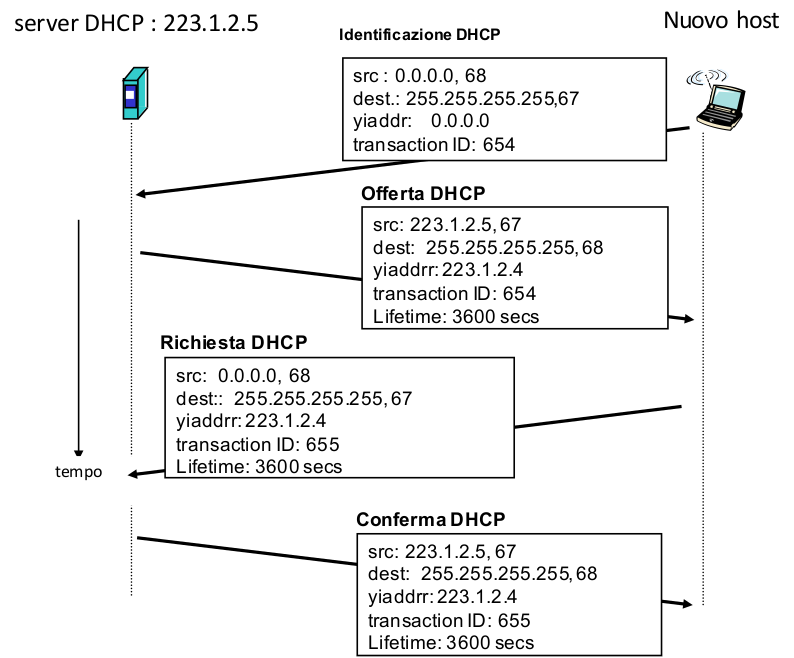
\includegraphics[scale=0.59]{livello_di_rete-img5.png}
\end{center}

\end{document}
